\documentclass[../DS07.tex]{subfiles}
\graphicspath{{./figures/}}

% \subimport{/home/nora/Documents/Enseignement/Prepa/bpep/exercices/DS/satellites_de_telecommunication/}{sujet.tex}

\begin{document}
\prblm[45]{Satellites de télécommunication\ifcorrige{~\small\textit{(D'après
			Mines-Ponts MP 2007)}}}

\enonce{
	On se propose d'étudier quelques aspects du fonctionnement de satellites de
	télécommunication en orbite autour de la Terre. Sauf mention contraire, on
	considérera que la Terre est une sphère homogène de masse $M_T$, de rayon
	$R_T$ et de centre $O$, immobile dans l'espace, sans rotation propre.
	\smallbreak
	On donne les valeurs numériques suivantes~:
	\begin{center}
		\renewcommand{\arraystretch}{1.5}
		\begin{tabular}{c|c|c}
			$\Gc $                              & $R_T$            & $M_T$              \\
			\hline
			\hline
			$\SI{6,67e-11}{m^3 kg^{-1} s^{-2}}$ & $\SI{6 370}{km}$ & $\SI{5,97e24}{kg}$ \\
		\end{tabular}
	\end{center}
}

\partie{Couverture d'un réseau de satellite}

\renewcommand{\version}{bonus}

\QR[][4]{
	\label{q:kepler}

	Un satellite de masse $M_S$ est en orbite circulaire de centre $O$, à une
	altitude $h=\SI{800}{km}$ . Établir la relation entre la période de révolution
	$T$ et $h$. Exprimer de même la relation entre la vitesse $v = \norm{\vec v}$
	et $h$ puis effectuer les applications numériques pour $T$ et $v$.

}{%
	Dans le référentiel géocentrique considéré comme galiléen on ne prend en
	compte que la force de gravitation exercée par la Terre $\vec f = -
		\cfrac{k}{r^2} \er$  avec $k=GM_TM_S$. On a de plus $r=R_T+h$.
	On peut ainsi appliquer le PFD au satellite dans le repère polaire $O, \er,
		\ez$~:
	\begin{align*}
		-M_Sr \tp^2 & = - \frac{k}{r^2}
		\\
		M_Sr \tpp = 0
	\end{align*}
	De la deuxième équation, on obtient $\tp = cste \Rightarrow v = r
		\tp = cste$. On peut ainsi ré-exprimer l'accélération radiale $a_r =
		- v^2/r$ d'où:
	\[
		M_S \frac{v^2}{r} = \frac{k}{r^2} \Rightarrow \boxed{v = \sqrt{\frac{GM_T}{R_T+h}}}
	\]
	De plus, on sait que $T = \frac{2\pi r}{v} \Rightarrow
		\boxed{\frac{T^2}{(R_T+h)^3} =\frac{4 \pi^2}{GM_T} }$. On retrouve ainsi la
	troisième loi de Kepler. Les A.N.s donnent $T=\SI{6.07e2}{s}$ et $v =
		\SI{7.46}{km.s^{-1}}$.
}

\QR[][1]{\label{q:viriel}
	Soient $\Ec_c$ et $\Ec_p$ l'énergie cinétique du satellite et son énergie
	potentielle dans le champ de gravitation de la Terre~; établir le «~théorème du
	viriel~»~: $2\Ec_c + \Ec_p = 0$.
}{%
	L'énergie potentielle a pour expression $\Ec_p(r) = -\cfrac{k}{r}$.
	On a $2\Ec_c + \Ec_p = M_S v^2 - \frac{G M_T M_S}{r} =  M_S \pa{ \frac{GM_T}{r} -
			\frac{G M_T }{r}} = 0$ d'où le résultat.
}

\enonce{\figCap{0.42}{schema}{\protect\label{fig:schema}
		\emph{$N$ est le pôle Nord et $S$ le pôle Sud. Satellite $P$, point $Q$ et
			ligne des horizons $AB$. Le plan orbital représenté est dit polaire (la
			ligne des pôles est N'S').}
	}
}

\QR[][3]{
	À chaque position $P$ du satellite correspond un point $Q$ sur la Terre à la
	verticale de ce point. L'ensemble des points $Q$ définit la trace de la
	trajectoire.
	\smallbreak
	Pour un observateur situé en $Q$, la durée de visibilité $\tau$ d'un satellite
	est l'intervalle de temps entre son apparition sur l'horizon (point $A$ de la
	Fig. \ref{fig:schema}) et sa disparition sous l'horizon (point $B$). Exprimer
	$\tau$ en fonction de $\varphi$ et $T$ puis montrer que
	%	\eq{
	%		\tau =  2\arccos\fracp{R_T}{R_T+h} \sqrt{\frac{(R_T+h)^3}{GM_T}}
	%	}
	\[
		\tau =  2\arccos\fracp{R_T}{R_T+h}\, f(h)
	\]
	et donner l'expression de $f(h)$.
	\smallbreak
	Réaliser l'application numérique toujours pour $h=\SI{800}{km}$.
}{%
	Il convient pour cela d'établir l'expression de l'angle $\varphi$ tel que
	$\cos(\varphi) = R_T/(R_T+h)$. La vitesse du satellite étant uniforme, on en
	déduit $\tau = \frac{2\varphi}{2\pi}T$ soit au final~:
	\[
		\boxed{
			\tau = 2\arccos\fracp{R_T}{R_T+h} \ub{\sqrt{\frac{(R_T+h)^3}{GM_T}}}{f(h)}
		}
	\]
	L'application numérique donne $\tau=\SI{9.2e2}{s}$
}

\QR[][2]{
	\label{q:train}
	Calculer $T/\tau$. Pour les besoins de la téléphonie mobile, on place sur des
	orbites polaires (c'est-à-dire contenues dans un plan méridien terrestre comme
	sur la figure~\ref{fig:schema}) un ensemble de satellites, identiques, appelé
	«~train de satellites ~».
	\smallbreak
	Ces satellites sont disposés régulièrement sur leur orbite polaire commune, à
	l'altitude de \SI{800}{km}. Calculer le nombre minimal de satellites
	nécessaires pour former un «~train~» afin que tous les points au sol, dans le
	même plan méridien que l'orbite, voient au moins un satellite à tout instant.
}{%
	\label{q:train}
	On a simplement $\cfrac{T}{\tau} = \cfrac{2\pi}{2\varphi} =
		\dfrac{\pi}{\arccos\fracp{R_T}{R_T+h}} \approx 6,6$. Le satellite est ainsi
	visible pendant $1/6,6$ ième de son trajet. Il faudra donc 7 satellites pour
	garantir la couverture permanente au sol (arrondi au supérieur).
}

\QR[][2]{
	Combien d'orbites polaires de ce type faut-il pour couvrir la surface de la
	Terre, c'est à dire pour que chaque point de la surface terrestre voie au
	moins un satellite à tout instant~? Combien doit-on disposer de satellites en
	tout~?
}{%
	D'après la question précédente, il faudrait aussi 7 «~trains de satellites~»
	pour couvrir toutes les longitudes. Cependant, un train de satellite couvre
	«~deux côtés~» et donc $\lfloor 7/2 \rfloor = 4$ trains suffisent. ce qui permet
	d'aboutir à un total de $7\times 4 = 28 $ satellites.
}

\QR[][3]{
	La prise en compte de la rotation de la Terre modifie le résultat de la
	question précédente. Dans cette question, on s'interroge sur la pertinence
	d'utiliser plutôt un satellite géostationnaire. Calculer la période et
	l'altitude d'un satellite placé sur orbite géostationnaire. La notion de durée
	de visibilité garde-t-elle, dans ce cas, un sens~? Quels sont les avantages et
	les inconvénients d'un satellite géostationnaire comparé au train de la
	question \ref{q:train}~?
}{%
	Sur l'orbite géostationnaire, la période de révolution du satellite vaut la
	période de révolution de la terre $T_T \approx \SI{86e3}{s}$.
	\smallbreak
	On peut utiliser la 3ième loi de Kepler~:
	%	\eq{
	%		\frac{T_T^2}{(R_T+h_g)^3} =\frac{4 \pi^2}{GM_T} \text{~~et~~} \frac{T^2}{(R_T+h)^3} =\frac{4 \pi^2}{GM_T} \Rightarrow \boxed{h_g =(R_T+h) \fracp{T_T}{T}^{2/3} - R_T \approx \SI{35700}{km}}
	%	}
	\[
		\frac{T_T^2}{(R_T+h_g)^3} =
		\frac{4 \pi^2}{GM_T} \qsoit
		\boxed{
			h_g=\pa{\cfrac{GM_TT_T^2}{4\pi^2}}^{1/3}-R_T
			\approx\SI{35700}{km}
		}
	\]

	La notion de «~visibilité~» est à prendre avec prudence~: pour un point du
	globe, le satellite est alors soit visible et la durée de visibilité est
	infinie, soit invisible. Il ne faut pas utiliser la formule de la question
	\ref{q:train} pour la durée de visibilité car on y faisait l'hypothèse d'une
	Terre immobile (le schéma permettant le calcul de $\varphi$ est incorrect dans
	ce cas~!~!). Pour une zone donnée de la Terre, il suffit de disposer d'un seul
	satellite au lieu d'une bonne quarantaine. Mais il est beaucoup plus éloigné,
	ce qui pose des problèmes de perte de transmission.
	\smallbreak
	Il faut aussi remarquer que les Pôles et les régions qui les entourent ne
	voient pas les satellites géostationnaires.
}

\partie{Influence des frottements aérodynamiques}

\QR[][4]{
La Terre est entourée d'une atmosphère qui s'oppose au mouvement du satellite.
La force de frottement $\vec f_a$ créée par l'atmosphère est proportionnelle
au carré de la vitesse $v$ du satellite et elle s'exprime par $\vec f_a =  -
	\alpha M_S v \vec v$, où $\alpha$ a une valeur positive, constante dans cette
question. Déterminer la dimension de $\alpha$ puis appliquer ensuite le
théorème de la puissance mécanique en supposant que le théorème du Viriel
établi à la question \ref{q:viriel} reste valable en présence de $\vec f_a$ .
En déduire finalement que~:
\begin{equation}
	\label{eq:h}
	\dv{h}{t} = -2 \alpha \sqrt{G M_T}\sqrt{R_T+h}
\end{equation}
}{%
On a $[F] = M.L.T^{-2} = [\alpha] M.L^2.T^{-2}$. On en déduit par identification
que $\boxed{[\alpha] = L^{-1}  }$.
\smallbreak
Le TPM appliqué au satellite donne~:
\[
	\dv{\Ec_c +\Ec_p}{t} = - \alpha M_S v^3 =  \frac{1}{2} \dv{\Ec_p}{t}
\]
De plus, $v^2 = 2\Ec_C/M_S = -\Ec_P/M_S = GM_T/(R_T+h)$. On en déduit en combinant
ces résultats que~:
\[
	- \alpha M_S \fracp{GM_T}{R_T+h}^{3/2} =
	\dot{h} \frac{GM_SM_T}{2(R_T+h)^2} \Rightarrow \dv{h}{t} =
	-2 \alpha \sqrt{G M_T}\sqrt{R_T+h}
\]
}

\QR[][4]{\label{q:chute}
	Un satellite placé sur une orbite d'altitude \SI{800}{km} subit une diminution
	d'altitude d'environ \SI{1}{m} par révolution~; sa vitesse est, en norme, très
	peu affectée au bout d'une révolution. En déduire une estimation au premier
	ordre de $\alpha$ (ne pas s'étonner de la petitesse extrême du résultat~!).
	Calculer, avec la même approximation, ce qu'il advient de l'altitude au bout
	de 10 ans de fonctionnement du satellite. Comparer à la solution exacte de
	l'équation (\ref{eq:h}) (obtenue par intégration de cette équation). Le fait
	d'avoir une augmentation de la vitesse en présence d'une force opposée au
	mouvement est-il paradoxal~?
}{%
	Entre le début et la fin de la révolution, $R_T+h$ n'a quasiment pas varié et
	on peut supposer ce terme constant (on note alors $h_0$ l'altitude initiale du
	satellite)~:
	\begin{gather*}
		\Delta h =
		- 2\alpha \ub{\Delta t}{=T} \sqrt{G M_T} \sqrt{R_T+h_0}
		\Rightarrow
		\alpha = - \frac{\Delta h}{2T\sqrt{GM_T}\sqrt{R_T+h_0}}
		\\\Leftrightarrow
		\boxed{
			\alpha =
			-\frac{\Delta h}{4\pi (R_T+h_0)^2} \approx
			\SI{1.53e-15}{m^{-1}}
		}
	\end{gather*}
	En dix années, on a effectué $n = \frac{\Delta T}{T} = 10 \frac{T_T}{T}\approx
		52000$ orbites donc au premier ordre (en supposant $\Delta h$ identique à
	chaque période), on a $\Delta h \approx -\SI{52}{km}$.
	\smallbreak
	Une résolution exacte de l'équation (à l'aide de la méthode de séparation des
	variables)~:
	\begin{align*}
		\frac{dh}{\sqrt{R_T+h}} & =
		-2\alpha\sqrt{GM_T} dt
		\Rightarrow
		2(\sqrt{R_T+h_1} - \sqrt{R_T+h_0}) =
		-2\alpha\sqrt{GM_T} \Delta T
		\\\Rightarrow
		\boxed{
			\Delta h = h_1- h_0 =
			\pa{\sqrt{R_T+h_0} - \alpha \sqrt{GM_T} \Delta T}^2 - R_T - h_0 \approx
			- \SI{51,3}{km}}
	\end{align*}
	Ce résultat est très proche de celui obtenu à l'aide de l'approximation. Il
	peut sembler surprenant qu'une force qui s'oppose au mouvement se concrétise
	par une augmentation de vitesse~: le freinage d'une voiture (force
	aérodynamique par exemple) réduit sa vitesse. Mais c'est sans compter sur
	l'énergie potentielle~: à une orbite plus basse correspond une vitesse plus
	élevée.
}

\QR[][4]{
En réalité, les frottements dépendent de la densité de l'atmosphère et donc de
l'altitude. Dans un certain domaine d'altitudes, $\alpha$ varie selon la loi
$\alpha(h)= \cfrac{\gamma}{h^\beta}$, où $\gamma$ et $\beta$ sont positifs.
Le même satellite que celui de la question \ref{q:chute} (perdant 1 mètre par
révolution pour $h \approx \SI{800}{km}$) perd, à l'altitude de \SI{400}{km},
2 mètres par révolution. Calculer $\gamma$ et $\beta$.
}{%
On observe que $\dv{h}{t} \propto \alpha(h)$, car les autres facteurs varient
peu. On en déduit ainsi que~:
\[
	\frac{\dv{h}{t}(h=h_{haut})}{\dv{h}{t}(h=h_{bas})} =
	\fracp{h_{bas}}{h_{haut}}^\beta =
	\frac{1/T_T}{2/T_T'}
	\Rightarrow
	\beta = \dfrac{\log(T_T'/(2T_T))}{\log(h_{bas}/h_{haut})}
\]
avec $T_T'$ la période de révolution à \SI{400}{km} d'altitude telle que
$T_T'/T=\fracp{R_T+h_{bas}}{R_T+h_{haut}}^{3/2} \approx 0,917$. On en déduit au
final $\beta \approx 1,13$ puis $\gamma = h_{haut}^\beta \times \alpha(h_{haut})
	\approx \SI{7,2e-9}{SI}$. En pratique, la valeur de $\gamma$ est très sensible
aux différents arrondis réalisés pour obtenir $\beta$ et seuls son ordre de
grandeur à du sens.
}

\partie[bonus]{Stabilisation de l'orientation d'un satellite par gradient de
	gravité}

\enonce[bonus]{
	\noindent
	\begin{minipage}[c]{.53\linewidth}
		La méthode de stabilisation d'attitude par gradient de gravité a été mise en
		œuvre pour les satellites artificiels afin qu'ils présentent vers la Terre
		toujours le même côté. Elle ne requiert aucune ressource d'énergie
		embarquée. Le principe de cette méthode a été établi par Lagrange, au
		XVIIème, afin d'expliquer pourquoi la Lune présente toujours la même face
		vers la Terre.
		\smallbreak
		\textbf{Modèle~:} le satellite est constitué de deux points matériels $M_1$
		et $M_2$ de masses identiques $m  =\frac{1}{2} M_S$ reliés par une tige
		rigide de masse nulle et de longueur $2l$.
		\smallbreak
		Le centre de masse $S$ du satellite décrit autour de la Terre une orbite
		circulaire uniforme de rayon $r_0 = R_T + h$ avec $l \ll r_0$. Le
		référentiel géocentrique $(R)$ lié au repère $(Oxyz)$ est supposé galiléen.
		\smallbreak
		On appelle $\th$ l'angle de $\vect{M_1M_2}$ avec l'axe $Ox'$ de $(R')$.
		On cherche à déterminer les éventuelles positions d'équilibre du satellite
		et leur stabilité. On suppose qu'il n'y a pas de frottements dans toute
		cette partie.
	\end{minipage}
	\hfill
	\begin{minipage}[c]{.43\linewidth}
		\vspace{0pt}
		\begin{center}
			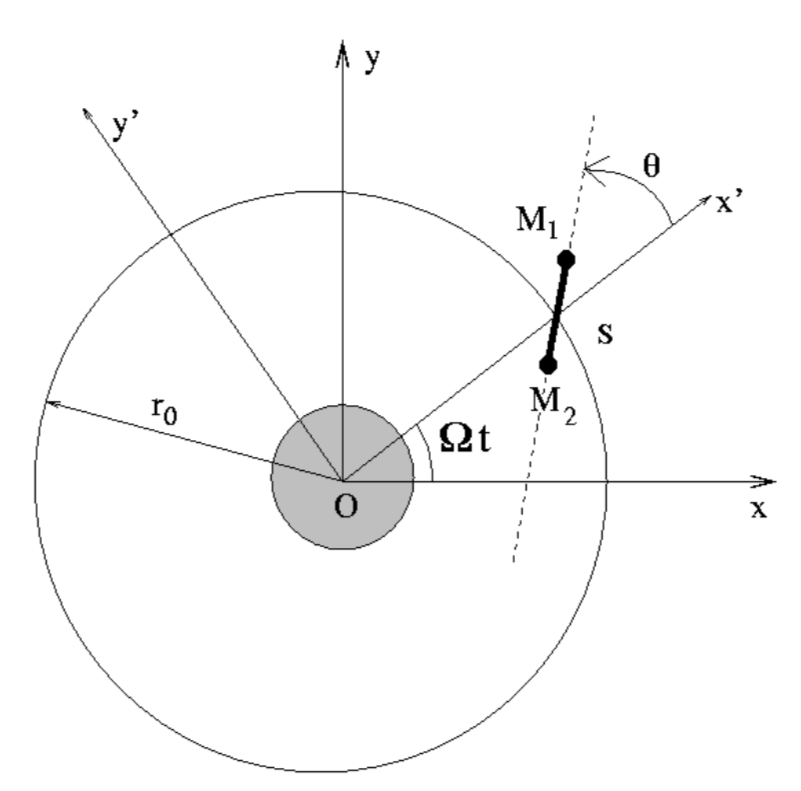
\includegraphics[width=\linewidth]{schema2}
			\captionof{figure}{Le satellite composé des points $M_1$ et $M_2$ reliés
				par une tige de longueur $2l$.}
			\label{fig:schema2}
		\end{center}
	\end{minipage}
}

\QR[bonus][2]{
	Exprimer les distances $r_1 = \norm{\vect{OM_1}}$ et $r_2 =
		\norm{\vect{OM_2}}$ en fonction de $r_0$, $l$ et $\th$
}{%
	On a $\vect{OM_1} = \vect{OS}+\vect{SM_1} \Rightarrow r_1 = \sqrt{r_0^2 + l^2
			+2r_0l \cos(\th)} $. De même, on trouve $r_2 = \sqrt{r_0^2 + l^2 -2r_0l
			\cos(\th)}$
}

\enonce[bonus]{
	On rappelle le développement limité à l'ordre 2 suivant~:
	\[
		\frac{1}{\sqrt{1+x}} = 1 - \frac{1}{2}x + \frac{3}{8}x^2 + o(x)
	\]
	De plus, on admet que l'énergie cinétique $\Ec_c$ du satellite s'exprime selon
	$\Ec_c = \frac{1}{2}M_s l^2\tp^2 $ (démonstration peu évidente dans
	le corrigé).
}

\siCorrige{
	\textbf{Démonstration~:}
	\smallbreak
	On a par définition $\Ec_c = \Ec_{c,1}+\Ec_{c,2} = \frac{1}{2}m (v_1^2 + v_2^2)$. De
	plus, on sait que $\vec v_1 = \dv{\vect{OM_1}}{t} = \dv{\vect{OS}}{t}
		+\dv{\vect{SM_1}}{t} = \vec v_g + l(\tp+\W) \vec e_{\th'}$
	puis que $\vec v_2 = \vec v_g - l(\tp+\W) \vec e_{\th'}$. On en
	déduit que~:
	\[
		\Ec_c =
		\frac{1}{2}m (2 v_g^2 + 2 l^2 \tp^2 +0)
		\Rightarrow
		\Ec_c =
		\frac{1}{2}M_S (r_0\W)^2 + \frac{1}{2}M_S l^2(\tp+ \W)^2
	\]
	\textbf{Remarques~: }
	\smallbreak
	\begin{itemize}
		\item Le vecteur $\vect SM_1$ tourne en effet à la vitesse angulaire $\W +
			      \tp$ par rapport au repère fixe dans $\Rc $ d'où le
		      résultat.
		\item Cependant, cette expression de l'énergie cinétique complique beaucoup la
		      suite du problème. En utilisant toutefois la conservation du moment
		      cinétique $L_0 =\pa{\vec{OM_1}\wedge m \vf _1 + \vec{OM_2}\wedge m
				      \vf _2}\cdot
			      \ez= M_Sr_0^2\W + M_Sl^2 (\W+\tp)$ implique $\dv{L_0}{t} =
			      0 \Rightarrow r_0^2 \dot{\W}  = -l^2 (\tpp + \dot{\W})$, on
		      peut établir que
		      \[
			      \dv{\Ec_c}{t} =
			      M_S r_0^2 \dot{\W}\W +
			      M_S l^2 (\tpp +
			      \dot{\W})(\tp +
			      \W) =
			      M_s l^2 \tp(\tpp+\dot{\W}) \approx
			      M_s l^2 \tp \tpp
		      \]
		      car $\dot{\W} = \frac{\tpp}{1+ (r_0/l)^2} \Rightarrow
			      \dot{\W} \ll \tpp$ (toujours via  l'expression du moment
		      cinétique).
		\item On peut alors ré-integrer cette relation pour obtenir~:
		      \[
			      \boxed{\Ec_c = \frac{1}{2}M_S l^2 \tp^2}
		      \]
		\item Ces résultats impliquent que le mouvement du centre de masse du
		      satellite n'est pas exactement uniforme. D'après la conservation du
		      moment cinétique, une variation de $\tp$ entraine une variation
		      de $\W$. Cette variation est toutefois très faible (de l'ordre de
		      $(l/r_0)^2$)
	\end{itemize}
}

\QR[bonus][4]{
	Montrer que l'énergie mécanique du système s'écrit en procédant aux
	approximations qui s'imposent ($l \ll r_0$)~:
	\[
		\Ec_m \approx
		- \frac{GM_TM_S}{r_0}
		\pa{1 +\frac{1}{2} \fracp{l}{r_0}^2 (3\cos^2(\th) -1)} +
		\frac{1}{2}M_S l^2 \tp^2
	\]
}{%
	On commence par s'intéresser aux termes d'énergie potentielle $\Ec_{p,i} = -k/r_i$
	avec $k = GM_T m$. On obtient ainsi en posant $\ep=l/r_0$:
	\begin{align}
		\Ec_{p,12} & =
		-\frac{k}{r_{12}} =
		-\frac{k}{\sqrt{r_0^2+l^2 \pm 2r_0l\cos(\th)}} =
		-\frac{k}{r_0} \frac{1}{\sqrt{1+\ep^2 \pm 2 \ep \cos(\th)}}
		\\\Leftrightarrow
		\Ec_{p,12} & =
		-\frac{k}{r_0}
		\pa{1 -
		\frac{1}{2} ( \ep^2 \pm 2 \ep\cos(\th) ) +
		\frac{3}{8} ( \ep^2 \pm 2 \ep\cos(\th) )^2} + o(\ep^2)
	\end{align}
	On peut maintenant ajouter les deux termes d'énergies potentielles (avec
	encore un terme quadratique à développer puis simplifier à droite du terme
	d'énergie potentielle)~:
	\[
		\Ec_{p,1} + \Ec_{p,2} = -\frac{k}{r_0} \pa{2 -\ep^2 +3 \ep^2 \cos^2(\th)} + o(\ep^2)
	\]
	On combine ensuite ce terme avec l'expression de l'énergie cinétique obtenue à
	la question précédente~:
	\[
		\Ec_m =
		\Ec_c + \Ec_p =
		-\frac{GM_TM_S}{r_0}
		\pa{1 +\frac{1}{2} \fracp{l}{r_0}^2 \pa{3 \cos^2(\th)-1}} +
		\frac{1}{2}M_S (l\tp)^2
	\]
	car $m=M_S/2$, d'où le résultat~!
}

\QR[bonus][4]{
	En déduire l'équation du mouvement. Indiquer les positions d'équilibre et
	préciser, pour celle(s) qui sont stable(s), la pulsation des petites
	oscillations autour de ces dernières. Conclure.
}{%
	On applique le TPM dans le référentiel géocentrique au satellite qui n'est
	soumis à aucune force non conservative. On en déduit~:
	\begin{gather*}
		\dv{\Ec_m}{t} = 0
		\Rightarrow
		- \frac{GM_T}{r_0} \fracp{l}{r_0}^2
		3\cos(\th)(-\sin(\th))\tp +
		l^2 \tp \tpp = 0
		\\\Rightarrow
		\tpp +
		\frac{3GM_T}{2r_0^3}\sin(2\th) = 0
		\Rightarrow
		\boxed{\tpp + 3 \W^2 \frac{\sin(2\th)}{2} = 0}
	\end{gather*}
	On est à l'équilibre lorsque $\tpp=0$ soit ici pour $\th=p
		\frac{\pi}{2},~p \in \mathbb{N}$.
	\begin{itemize}
		\item Pour $\th = 0+x$ avec $x<<1$, on a comme équation du mouvement $
			      \xpp + 3\W^2 x = 0$ qui est l'équation de l'oscillateur harmonique
		      donc la position d'équilibre est stable et la pulsation des petites
		      oscillations vaut $\w_0 = \W\sqrt{3}$
		\item Pour $\th = \pi/2+x$, on a maintenant $\xpp- \w_0^2 x$.
		      Cette position d'équilibre n'est pas stable.
		\item Pour $\th = \pi+x$, on a $\xpp + \w_0^2 x=0$ et on retrouve
		      la même équation que pour la première position d'équilibre. Cette position
		      d'équilibre est donc aussi stable et de pulsation $\w_0$
		\item Pour $\th = 3\pi/2+x$, on obtient au final $\xpp- \w_0^2
			      x$~: équilibre instable.
	\end{itemize}
	Ainsi, seules les positions verticale (à l'endroit ou à l'envers) sont
	stables. En cas de léger décalage, le satellite va donc osciller autour de la
	position d'équilibre verticale et donc toujours présenter le même côté vers la
	Terre.
}
\end{document}
